\chapter{Evaluation}
This chapter discusses the process of testing the framework and evaluating the same.  The scope of the evaluative is to ensure the feasibility of the proposed approach and measure the effort involved in extending the framework to create new ITS application and simulate it.  For testing two scenarios simulation and each scenario is based on a different application.  An overview of the testing infrastructure is discussed before explaining the scenarios.
\section {Test Setup}
For testing, a distributed network is built. The  Carla server runs in a machine located at the Trinity College Dublin Linux lab at South Leinster Street. To run the Client (i.e. to spawn the actors) an AWS Linux EC2 instance and Lenovo laptop were used and a separate Linux EC2 instance to run CarlaViz server. 

In both, the scenario, three vehicles and three roadside unit were spawned from two client nodes (i.e., two RSU and one vehicle form EC2 instance and two vehicles and one RSU from the laptop). The figure illustrates the entire setup. 

 \begin{figure}[h!]
    \centering
    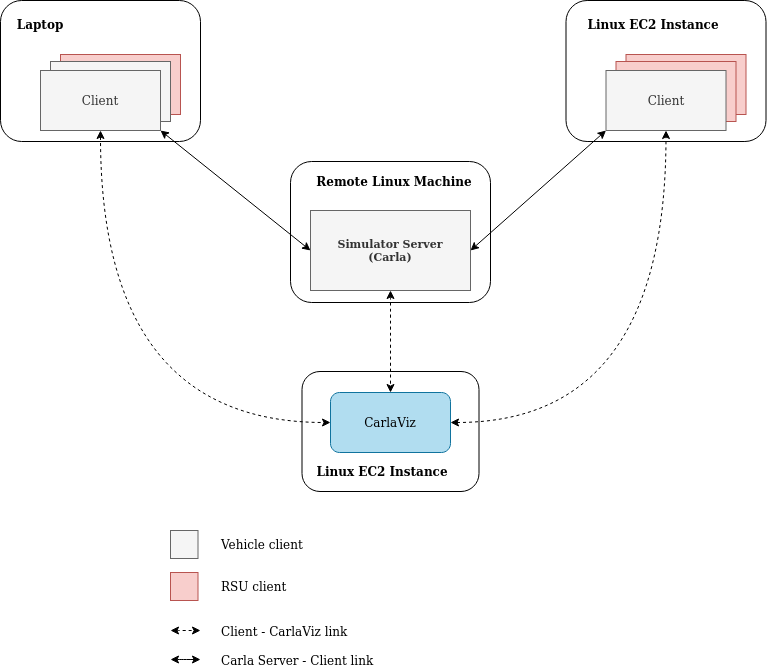
\includegraphics[width=11cm]{Framework/Images/testSetup.png}.
    \caption{Test Setup}
    \label{sequence}
\end{figure}

\section{Scenario}
\subsection{CAM Exchange}
The motive for simulating this scenario is to test the performance of the communication module to establish vehicular communication between vehicle and RSU. In this scenario, the CAM message is exchanged between all the actors. Once received, the actor displays the message using the CarlaViz \say{draw\_text} function. The content for the CAM message used in this scenario is a string combining the actor's \say{role\_name} and \say{id} attribute. The code snippets of this scenario is available in appendix.

\subsubsection{Implementation}
\begin{itemize}
    \item To create a custom behaviour for RSU to broadcast its \say{role\_name} and \say{id} attribute as CAM and to display the received message using CarlaViz, \say{CamRSU} behaviour class is created by inheriting \say{BaseRsuAgent} class and then override the \say{BaseBehaviour} class with \say{CamRSU} by adding the decorator \say{@rsuAgent}.

    \item To make the vehicles receive the CAM, \say{CaMsgHandler} class is created by inheriting \say{BaseRxHandler} class and added to the framework using \say{@addRxHandler}.

    \item To create a custom behaviour for Vehicles to broadcast its \say{role\_name} and \say{id} attribute as CAM and to display the received message using CarlaViz, \say{CamVehicle} behaviour class is created by inheriting \say{BaseVehicleAgent} class and then override the \say{BaseBehaviour} class with \say{CamVehicle} by adding the decorator \say{@rsuAgent}.

\end{itemize}


\subsection{DENM Exchange}
The motive of this scenario is to create a sample ITS safety application that sends hazard warnings. It sends lane status and speed limit messages. Two RSU broadcast the lane status message and the third broadcast the speed limit message. In this scenario, vehicles behave according to the DENM it receives from the RSU. The path and speed of the vehicle is visualized using CarlaViz to evaluate the behaviour. The code snippets of this scenario is available in appendix.
\subsubsection{Implementation}
\begin{itemize}
    \item To create a custom behaviour for RSU to broadcast lanchange and speed limit messages as DENM, \say{DenmRSU} behaviour class is created by inheriting \say{BaseRsuAgent} class and then override the \say{BaseBehaviour} class with \say{DenRSU} by adding the decorator \say{@rsuAgent}. As three RSU broadcast different message all have different behaviour and three classes are created.

    \item To make the vehicles receive the DENM, \say{DenMsgHandler} class is created by inheriting \say{BaseRxHandler} class and added to the framework using \say{@addRxHandler}.

    \item To create a custom behaviour for a vehicle to receive DENM and act accordingly and visualize its path and speed using CarlaViz, \say{DenmVehicle} behaviour class is created by inheriting \say{BaseVehicleAgent} class and then override the \say{BaseBehaviour} class with \say{DenmVehicle} by adding the decorator \say{@rsuAgent}.

\end{itemize}

\section{Discussion}
Since the framework does not have an evaluation component, visualization provided by the CarlaViz is used to evaluate both the scenarios.  

The screenshots of  DENM scenarios in the appendix shows the message exchange and cooperation between actors. The basic aspect of  ITS  is to improve the safety and driving experience by establishing cooperation among the traffic. Thus based on the screenshots of the scenario visualization and the test setup made, we can conclude that the proposed method is feasible to perform a distributed ITS simulation. 

The decorator design pattern followed in the framework helps it to extend it without altering the flow and behaviour of the. The developer has to create handlers and behaviour classes according to their need. This approach allows developers to create an ITS application with a little knowledge about the framework. Thus we can conclude, the framework can be easily extended.
